\documentclass[10pt, a4paper, hidelinks]{article}
\usepackage[paper=a4paper, left=2cm, right=2cm, bottom=2cm, top=3cm]{geometry} %ajustar márgnens
\usepackage[latin1]{inputenc}
\usepackage[spanish]{babel}
\usepackage{caratula}
\usepackage{enumitem} 
\usepackage{hyperref}
\usepackage{mathtools}
\usepackage[font=small,labelfont=bf]{caption}
\newcommand\floor[1]{\lfloor#1\rfloor}
\newcommand\ceil[1]{\lceil#1\rceil}
%\usepackage{clrscode3e} Estilo Cormen
\usepackage[spanish,onelanguage,ruled,vlined,nofillcomment]{algorithm2e}
\usepackage{algpseudocode}
\usepackage{xcolor}
\usepackage[final]{pdfpages} % para agregar el enunciado
%%%%%%%%%%%%%% Formato de párrafos %%%%%%%%%%%%%%%%%%
\setlength{\parindent}{2em}
\setlength{\parskip}{3pt}
%%%%%%%%%%%%%%%%%%%%%%%%%%%%%%%%%%%%%%%%%%%%%%%%%%%%%%%
\usepackage{fancyhdr}
\usepackage{lastpage}
\setlength{\intextsep}{0.2cm}
\pagestyle{fancy}
\lhead{Sistemas Operativos}
\rhead{$1^{\mathrm{er}}$ cuatrimestre de 2018}

\LinesNumbered
\DontPrintSemicolon

\newcommand{\comp}[1]{$\mathcal{O}(#1)$}

%%%%%%%%%%%%%%%%%%% Macro para comentar codigo %%%%%%%%%%%%%%%%%%%%%%%%%
\newcommand{\comentario}[1]{
\SetKwComment{Comment}{/* }{ */}
\textcolor{blue}{\Comment*[h]{{#1}}}
}
%%%%%%%%%%%%%%%%%%%%%%%%%%%%%%%%%%%%%%%%%%%%%%%%%%%%%%%%%%%%%%%%%%%%%%%%

\begin{document}

\materia{Sistemas Operativos}
\submateria{Primer cuatrimestre del 2018}
\titulo{Trabajo Práctico 2: \texttt{blockchain}}
\integrante{Budiño, Gabriel Fabricio}{046/16}{gabriel.f.budi@gmail.com} % obligatorio 
\integrante{Garro, Damián Eugenio}{354/16}{damian.garro.mst@gmail.com} % obligatorio 
\integrante{Rozenberg, Uriel Jonathan}{838/12}{rozenberguriel@gmail.com} % obligatorio 

\maketitle

\tableofcontents
\pagenumbering{gobble}

\pagebreak
\pagenumbering{arabic}
\cfoot{\thepage /\pageref{LastPage}}

\section{Introducción}
Para este trabajo se debía implementar una cadena de bloques ($blockchain$) utilizando la interfaz MPI con el objetivo de desarrollar conocimientos en sistemas distribuidos.

A continuación se presenta un breve resumén de la resolución de cada ejercicio así como de la experimentación realizada. El enunciado completo se encuentra en el Apéndice A, donde puede consultarse tanto la información de las estructuras usadas como los enunciados a los que responden las siguientes secciones del informe.

\section{Resolución}
\subsection{Ejercicio 1}
La función \texttt{broadcast\_block} es la encargada de, al momento en que un nodo mina exitosamente un bloque, comunicárselo al resto. El pseudocódigo de la misma es el siguiente:

\begin{algorithm}[H]
\SetKwProg{Fn}{Función}{}{fin}
\SetAlgoLined
\Fn{broadcast\_block(bloque)}{
	\ForEach{nodo n distinto del productor del bloque}{
		\texttt{MPI\_Send}($bloque$, $n.rank$, \texttt{TAG\_NEW\_BLOCK}) \\
	}
}
\caption{\texttt{broadcast\_block}}
\end{algorithm}

Para referenciar a un proceso ($nodo$) usamos su \texttt{rank} dentro del communicator global \texttt{MPI\_COMM\_WORLD}. Cada nodo metiene las variables \texttt{mpi\_rank} y \texttt{total\_nodes}. Así, para cada 1 $\leq i \leq$ \texttt{total\_nodes}, definimos $destino$ como $(i + \texttt{mpi\_rank})$ $mod$ \texttt{total\_nodes} y enviamos el mensaje usando \texttt{MPI\_Send} con $destino$, $bloque$ y el tag \texttt{TAG\_NEW\_BLOCK} como parámetros (principalmente). Es decir, enviamos el bloque desde el nodo siguiente al que lo minó en adelante, asegurándonos así que todos los nodos envíen mensajes en distinto orden.
 
\subsection{Ejercicio 2}
Para la resulución de este ejercicio, se agregó a la información que mantiene cada nodo un bool atómico \texttt{probando}. Además, se implementaron las funciones \texttt{lock} y \texttt{unlock} como se muestran a continuación:

\begin{algorithm}[H]
\SetKwProg{Fn}{Función}{}{fin}
\SetAlgoLined
\Fn{lock()}{
	$expected$ $\leftarrow$ \texttt{false} \\
	\While{$\lnot$ \texttt{probando}.compare\_exchange\_weak($expected$, \texttt{true})}{
		$expected$ $\leftarrow$ \texttt{false}
	}
}
\caption{\texttt{lock}}
\end{algorithm}

\begin{algorithm}[H]
\SetKwProg{Fn}{Función}{}{fin}
\SetAlgoLined
\Fn{unlock()}{
	\texttt{probando} $\leftarrow$ \texttt{false}
}
\caption{\texttt{unlock}}
\end{algorithm}

\textbf{TODO: Creo que no hace faltan esos pseudocódigos, decir que implementamos un spinlock.}

Se pedía modificar las funciones \texttt{node} y \texttt{proof\_of\_work} para evitar $race$ $conditinos$. A continuación, se muestra el pseudocódigo de la parte implementada del método \texttt{node}:

\begin{algorithm}[H]
\SetKwProg{Fn}{Función}{}{fin}
\SetAlgoLined
\Fn{node()}{
	\comentario{Tomar valor de mpi\_rank y de total\_nodes} \\
	\comentario{Inicialización del primer bloque} \\
	\comentario{Crear thread para minar} \\
	crear nuevo thread con la función \texttt{proof\_of\_work} como punto de inicio \\
	\While{\texttt{true}}{
		\comentario{Recibir mensajes de otros nodos} \\
		$status$ $\leftarrow$ \texttt{MPI\_Probe()} \\
		\comentario{Si es un mensaje de nuevo bloque} \\
		\If{status.tag = \texttt{TAG\_NEW\_BLOCK}}{
			$status$ $\leftarrow$ \texttt{MPI\_Recv($block$)} \\
			\texttt{lock()} \\
			\texttt{validate\_block\_for\_chain}($block$, $status$) \\
			\texttt{unlock()}
		} \comentario{Si es un mensaje de pedido de cadena} \\
		\ElseIf{status.tag = TAG\_CHAIN\_HASH}{
			$status$ $\leftarrow$ \texttt{MPI\_Recv($block_hash$)} \\
			\texttt{mandar\_cadena}($block_hash$, $status$) \\
		}
	}
}
\caption{\texttt{node}}
\end{algorithm}

Ya que el mensaje recibido puede contener un bloque minado por otro o un hash para solicitar una cadena, y estos tienen tipos diferentes, antes de llamar a la función \texttt{MPI\_Recv} se llama a \texttt{MPI\_Probe()} para verificar el $tag$ del próximo mensaje recibido y a partir de éste usar \texttt{MPI\_Recv} con el tipo de dato correcto.

Si se recibe un mensaje con $tag$ \texttt{TAG\_CHAIN\_HASH} entonces se invoca a la función \texttt{mandar\_cadena} que manda la cadena al nodo que la solicitó. Para eso, la misma crea un arreglo de bloque cuyo tamaño (en cantidad) es el mínimo entre \texttt{VALIDATION_BLOCKS} y el índice del bloque del hash solicitada. A continuación llena el arreglo, en la primera posición con el bloque del hash recibido y en las siguientes con los bloques anteriores. Los bloques los obtiene usando el diccionario \texttt{node\_blocks}.

En cuanto a la función \texttt{proof\_of\_work}, una vez que se consigue la cantidad de ceros requerida por la dificultad configurada, se ejecuta un bloque que inicialmente verifica que no haya cambiado \texttt{last\_block\_in\_chain} y finalmente llama a \texttt{broadcast\_block} para comunicar que se ha minado un bloque. Consideramos estas dos acciones como los límites de la sección crítica, así que llamamos a \texttt{lock()} inmediatamente antes de la primera y a \texttt{unlock()} inmediatamente después de la segunda, de esta forma evitamos \textit{race conditions} porque la cadena del nodo solo puede ser modificada por un \textit{thread} al mismo tiempo

\textbf{TODO: Detallar acá \texttt{mandar\_cadena}? Pero antes ver lo de recibir hash en vez de bloque. Ver si hacemos lo de probe, el pseudcódigo puede ser más pseudo.}

\subsection{Ejercicio 3}
Cuando un nodo mine un nuevo bloque y le avise al resto, estos deberán decidir si agregarlo o no a la cadena. Para eso se utiliza la función \texttt{validate\_block\_for\_chain}, la cual debía cumplir con el consenso definido en la sección 3 del enunciado. Su pseudocódigo es el siguiente:

\begin{algorithm}[H]
\SetKwProg{Fn}{Función}{}{fin}
\SetAlgoLined
\Fn{validate\_block\_for\_chain(rBlock, status)}{
	\If{\texttt{valid\_new\_block(rBlock)}}{
		agrego $rBlock$ a \texttt{node\_blocks} \\
		\If{rBlock.indice = 1 y \texttt{last\_block\_in\_chain}.indice = 0}{
			\comentario{2do item del consenso} \\
			\texttt{last\_block\_in\_chain} $\leftarrow$ $rBlock$ \\
			devolver \texttt{true}
		}
		\If{rBlock.indice = \texttt{last\_block\_in\_chain}.indice + 1}{
			\uIf{anterior de rBlock = anterior de \texttt{last\_block\_in\_chain}}{
				\comentario{3er item del consenso} \\
				\texttt{last\_block\_in\_chain} $\leftarrow$ $rBlock$ \\
				devolver \texttt{true} \\			
			} \Else {
				\comentario{4to item del consenso} \\ 
				devolver \texttt{verificar\_y\_migrar\_cadena}($rBlock$, $status$)
			}
		}
		\If{rBlock.indice = \texttt{last\_block\_in\_chain}.indice}{
			\comentario{5to item del consenso} \\
			devolver \texttt{false}		
		}
		\If{rBlock.indice $<$ \texttt{last\_block\_in\_chain}.indice}{
			devolver \texttt{false}		
		}
		\If{rBlock.indice $>$ \texttt{last\_block\_in\_chain}.indice}{
			\comentario{6to item del consenso} \\
			devolver \texttt{verificar\_y\_migrar\_cadena}($rBlock$, $status$) \\
		}
	}
	\comentario{1er item del consenso} \\
	devolver \textit{false}
}
\caption{\texttt{validate\_block\_for\_chain}}
\end{algorithm}

Esta función puede modificar \texttt{last\_block\_in\_chain} a salvo de \textit{race conditions} porque se llama dentro de la sección crítica que definimos en el ejercicio anterior. 

\textbf{TODO: Hablar quizás del if que no esta en el consenso.}
 
\subsection{Ejercicio 4}
Llegado al caso donde un nodo deba migrar a la $blockchain$ de otro, se utilizará la función \texttt{verificar\_y\_migrar\_cadena}. La misma debía cumplir con el protocolo descripto en la sección 4 del enunciado. A continuación se muestra su pseudocódigo:

\begin{algorithm}[H]
\SetKwProg{Fn}{Función}{}{fin}
\SetAlgoLined
\Fn{\texttt{verificar\_y\_migrar\_cadena}(rBlock, status)}{
	\comentario{Solicitud de los bloques} \\	
	\texttt{MPI\_Send}($rBlock.hash$, $status.mpi\_source$, \texttt{TAG\_CHAIN\_HASH}) \\
	\comentario{Recepción de los bloques} \\
	$blockchain$ $\leftarrow$ nuevo arreglo de bloques \\
	\texttt{MPI\_Recv}($blockchain$, $status.mpi\_source$, \texttt{TAG\_CHAIN\_RESPONSE}) \\
	\comentario{1er item del protocolo} \\
	\If{el primer elemento de $blockchain$ tiene índice o hash distinto al pedido}{
		devolver \texttt{false}	
	}
	\ForEach{bloque b $\in$ blockchain}{
		\comentario{2do item del protocolo} \\
		\If{el hash de b es válido}{
			devolver \texttt{false}	
		}
		$b'$ $\leftarrow$ siguiente del bloque b en blockchain \\
		\comentario{3er item del protocolo} \\		
		\If{hash del anterior de b $\neq$ b'.hash}{
			devolver \texttt{false}			
		}
		\comentario{4to item del protocolo} \\
		\If{b.indice $\neq$ b'.indice + 1}{
			devolver \texttt{false}		
		}	
	}
	$u$ $\leftarrow$ ultimo bloque de $blockchain$ \\
	\If{ningún b $\in$ blockchain está en el diccionario $\land$ $u$.indice $\neq$ 1}{
		devolver \texttt{false}		
	}
	agregar bloques recibidos a \texttt{node\_blocks} \\
	\texttt{last\_block\_in\_chain} $\leftarrow$ $blockchain$[0] \\
	devolver \texttt{true}	
}
\caption{\texttt{verificar\_y\_migrar\_cadena}}
\end{algorithm}

El arreglo $blockchain$ se crea con tamaño \texttt{VALIDATION_BLOCKS} y en \texttt{MPI\_Recv} se especifica este valor para la cantidad máxima de bloques recibidos. Sin embargo, se pueden recibir menos y por eso utilizamos la función \texttt{MPI_Get_count} para saber la cantidad de bloques recibida. 

En cuanto al segundo ítem de verificaciones del conceso, el enunciando especifica que "El hash del bloque recibido es igual al calculado por la función \texttt{block\_to\_hash}.". Lo que hicimos en cambio fue revisar que el hash además resuelva el problema usando la función \texttt{solves\_problem}, y la verificación la hacemos para todos los blqoues recibidos, no solo uno.

Esta función se llama solo desde la \texttt{validate\_block\_for\_chain}, la cual ya dijimos que se ejecuta dentro de la sección crítica, así que no hay \textit{race conditions} con el \textit{thread} que mina bloques.

\subsection{Ejercicio 5}

\section{Experimentación}


\newpage
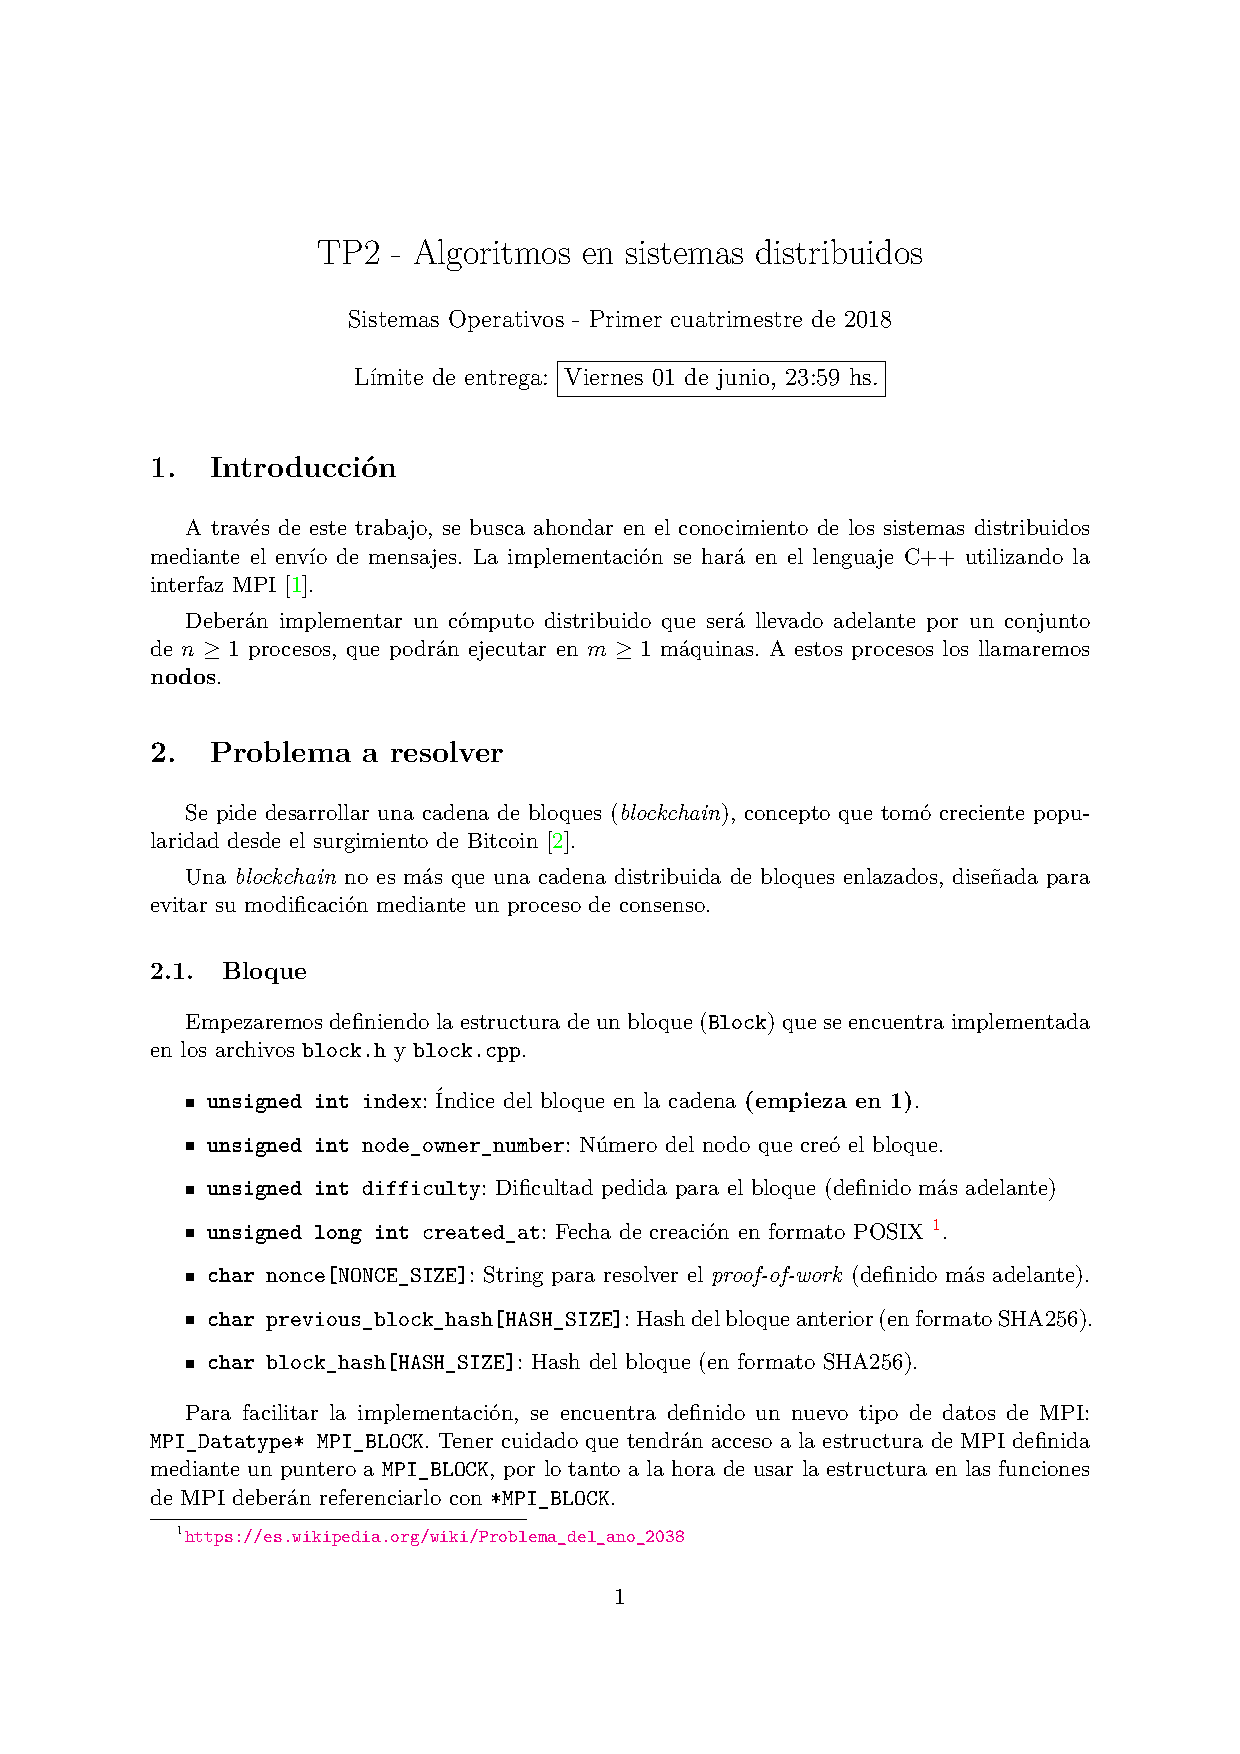
\includepdf[scale=0.75,pages=1,pagecommand=\section{Apéndices}
\subsection{Apéndice A - Enunciado}]{../enunciado.pdf}
\includepdf[scale=0.75,pages=2-,pagecommand=]{../enunciado.pdf}

\subsection{Apéndice B - Aclaraciones}

\end{document}

